\section{Fourier Series}

\begin{conceptbox}
    Fourier series represent periodic functions as sums of simple sinusoidal functions. The central idea is that a sufficiently well-behaved periodic function can be decomposed into harmonically related sine and cosine waves.

    For a function with period $2L$, the Fourier series is written as
    \[
        f(x)=\frac{a_0}{2}+\sum_{n=1}^{\infty}
        \left[
            a_n\cos\left(\frac{n\pi x}{L}\right)
            +b_n\sin\left(\frac{n\pi x}{L}\right)
            \right].
    \]
\end{conceptbox}

Fourier series extend the idea of representing a complicated object using simpler building blocks. In vector spaces, we express a vector as a combination of basis vectors. In Fourier analysis, we express a periodic function as a combination of orthogonal basis functions:
\[
    1,\quad \cos\left(\frac{\pi x}{L}\right),\quad \sin\left(\frac{\pi x}{L}\right),\quad
    \cos\left(\frac{2\pi x}{L}\right),\quad \sin\left(\frac{2\pi x}{L}\right),\quad \ldots
\]

The connection to previous topics is important. From vectors and inner products, we know that orthogonality allows clean decomposition. From series, we know that infinite sums can approximate functions. Fourier series combines both ideas.

\begin{noteBox}
    In engineering, Fourier series are used to analyze vibrations, sound waves, alternating current signals, heat conduction, communication signals, filters, and periodic mechanical motion. Instead of studying a complicated waveform directly, we study its frequency components.
\end{noteBox}

\subsection{Trigonometric Fourier Series}

\subsubsection*{Motivation and Intuition}

Many engineering signals repeat. Examples include AC voltage, rotating machinery vibration, periodic forcing functions, sound waves, and repeated pulse trains.

A periodic function may look complicated in the time domain, but it can often be understood as a combination of a constant component, a fundamental sinusoid, and higher harmonics.

\begin{conceptbox}
    If $f(x)$ has period $2L$, its trigonometric Fourier series is
    \[
        f(x)=\frac{a_0}{2}+\sum_{n=1}^{\infty}
        \left[
            a_n\cos\left(\frac{n\pi x}{L}\right)
            +b_n\sin\left(\frac{n\pi x}{L}\right)
            \right],
    \]
    where
    \[
        a_0=\frac{1}{L}\int_{-L}^{L} f(x)\,dx,
    \]
    \[
        a_n=\frac{1}{L}\int_{-L}^{L}
        f(x)\cos\left(\frac{n\pi x}{L}\right)\,dx,
        \qquad n=1,2,3,\ldots
    \]
    and
    \[
        b_n=\frac{1}{L}\int_{-L}^{L}
        f(x)\sin\left(\frac{n\pi x}{L}\right)\,dx,
        \qquad n=1,2,3,\ldots
    \]
\end{conceptbox}

\subsubsection*{Geometric Interpretation}

The coefficients $a_n$ and $b_n$ measure how much of each cosine and sine wave is present in $f(x)$. This is similar to projecting a vector onto basis vectors.

The constant term $\frac{a_0}{2}$ represents the average or DC component of the function.

\begin{conceptbox}
    The functions
    \[
        1,\quad \cos\left(\frac{n\pi x}{L}\right),\quad
        \sin\left(\frac{n\pi x}{L}\right)
    \]
    are orthogonal on $[-L,L]$. This orthogonality is what allows each Fourier coefficient to be computed independently.
\end{conceptbox}

\subsubsection*{Key Properties}

If $f(x)$ satisfies Dirichlet-type conditions on $[-L,L]$, then its Fourier series converges to
\[
    f(x)
\]
at points where $f$ is continuous, and to
\[
    \frac{f(x^+)+f(x^-)}{2}
\]
at jump discontinuities.

\begin{noteBox}
    At a discontinuity, the Fourier series does not choose the left-hand value or the right-hand value. It converges to the average of the two limiting values. This is important when analyzing square waves, pulse signals, and switching circuits.
\end{noteBox}

\subsubsection*{Determining Whether a Function is Even or Odd}

\begin{conceptbox}
    To determine whether a function is even or odd, replace $x$ with $-x$ and simplify.

    A function is \textbf{even} if
    \[
        f(-x)=f(x).
    \]

    A function is \textbf{odd} if
    \[
        f(-x)=-f(x).
    \]

    If neither condition is satisfied, then the function is \textbf{neither even nor odd}.
\end{conceptbox}

Geometrically, an even function is symmetric about the $y$-axis. This means the left side of the graph is a mirror image of the right side.

An odd function is symmetric about the origin. This means that if the graph is rotated $180^\circ$ about the origin, it looks the same.

\begin{examplebox}
    Determine whether
    \[
        f(x)=x^2
    \]
    is even or odd.

    Replace $x$ with $-x$:
    \[
        f(-x)=(-x)^2.
    \]

    Simplify:
    \[
        f(-x)=x^2.
    \]

    Since
    \[
        f(-x)=f(x),
    \]
    the function is \textbf{even}.

    \begin{center}
        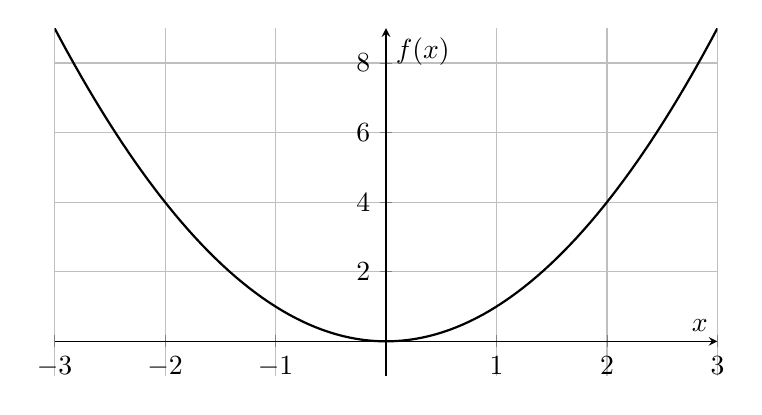
\begin{tikzpicture}
            \begin{axis}[
                    axis lines=middle,
                    xlabel={$x$},
                    ylabel={$f(x)$},
                    xmin=-3, xmax=3,
                    ymin=-1, ymax=9,
                    grid=both,
                    width=10cm,
                    height=6cm,
                    samples=100,
                    domain=-3:3
                ]
                \addplot[thick] {x^2};
            \end{axis}
        \end{tikzpicture}
    \end{center}
    The graph is symmetric about the $y$-axis.
\end{examplebox}

\begin{examplebox}
    Determine whether
    \[
        f(x)=x^3
    \]
    is even or odd.

    Replace $x$ with $-x$:
    \[
        f(-x)=(-x)^3.
    \]

    Simplify:
    \[
        f(-x)=-x^3.
    \]

    Since
    \[
        f(-x)=-f(x),
    \]
    the function is \textbf{odd}.

    \begin{center}
        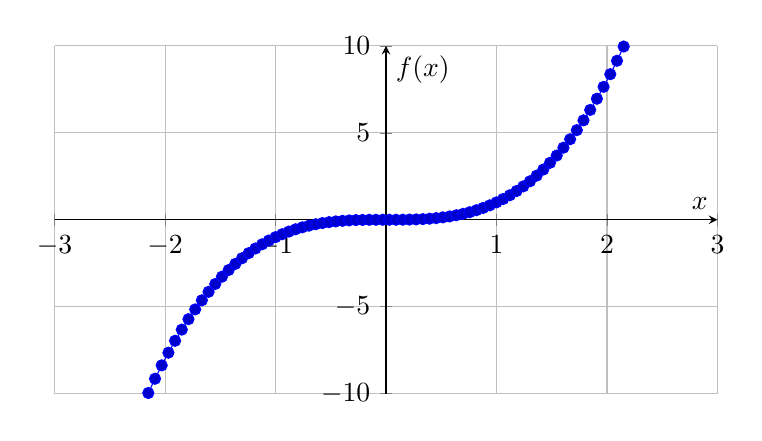
\begin{tikzpicture}
            \begin{axis}[
                    axis lines=middle,
                    xlabel={$x$},
                    ylabel={$f(x)$},
                    xmin=-3, xmax=3,
                    ymin=-10, ymax=10,
                    grid=both,
                    width=10cm,
                    height=6cm,
                    samples=100,
                    domain=-3:3
                ]
                \addplot {x^3};
            \end{axis}
        \end{tikzpicture}
    \end{center}

    The graph is symmetric about the origin.
\end{examplebox}

\begin{examplebox}
    Determine whether
    \[
        f(x)=x+1
    \]
    is even, odd, or neither.

    Replace $x$ with $-x$:
    \[
        f(-x)=-x+1.
    \]

    Compare with $f(x)$:
    \[
        f(x)=x+1.
    \]

    Since
    \[
        -x+1\neq x+1,
    \]
    the function is not even.

    Now compare with $-f(x)$:
    \[
        -f(x)=-(x+1)=-x-1.
    \]

    Since
    \[
        -x+1\neq -x-1,
    \]
    the function is not odd.

    Therefore,
    \[
        f(x)=x+1
    \]
    is \textbf{neither even nor odd}.

    \begin{center}
        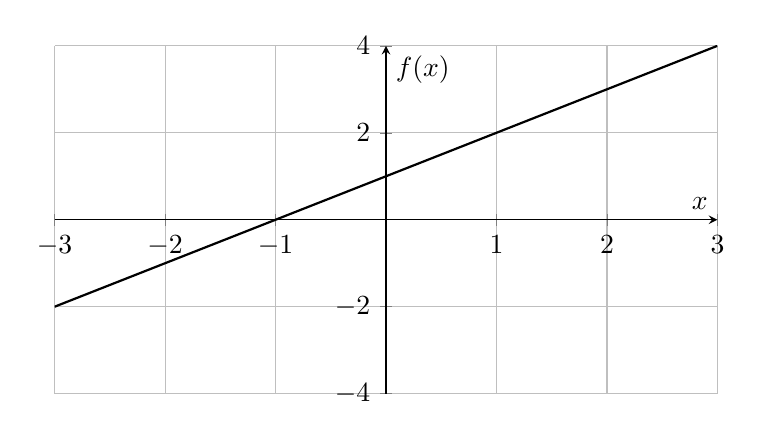
\begin{tikzpicture}
            \begin{axis}[
                    axis lines=middle,
                    xlabel={$x$},
                    ylabel={$f(x)$},
                    xmin=-3, xmax=3,
                    ymin=-4, ymax=4,
                    grid=both,
                    width=10cm,
                    height=6cm,
                    samples=100,
                    domain=-3:3
                ]
                \addplot [thick] {x+1};
            \end{axis}
        \end{tikzpicture}
    \end{center}

    The graph is not symmetric about the $y$-axis and is not symmetric about the origin.
\end{examplebox}

\subsubsection*{Worked Example}

\begin{examplebox}
    Find the Fourier series of
    \[
        f(x)=x,\qquad -\pi<x<\pi.
    \]

    Here, the period is $2\pi$, so $L=\pi$. The Fourier series has the form
    \[
        f(x)=\frac{a_0}{2}+\sum_{n=1}^{\infty}
        \left[a_n\cos(nx)+b_n\sin(nx)\right].
    \]

    First compute $a_0$:
    \[
        a_0=\frac{1}{\pi}\int_{-\pi}^{\pi}x\,dx.
    \]
    Since $x$ is an odd function,
    \[
        \int_{-\pi}^{\pi}x\,dx=0.
    \]
    Thus,
    \[
        a_0=0.
    \]

    Next compute $a_n$:
    \[
        a_n=\frac{1}{\pi}\int_{-\pi}^{\pi}x\cos(nx)\,dx.
    \]
    Since $x$ is odd and $\cos(nx)$ is even, their product is odd:
    \[
        x\cos(nx)\text{ is odd}.
    \]
    Therefore,
    \[
        a_n=0.
    \]

    Now compute $b_n$:
    \[
        b_n=\frac{1}{\pi}\int_{-\pi}^{\pi}x\sin(nx)\,dx.
    \]
    Since $x$ is odd and $\sin(nx)$ is odd, their product is even:
    \[
        x\sin(nx)\text{ is even}.
    \]
    Thus,
    \[
        b_n=\frac{2}{\pi}\int_0^\pi x\sin(nx)\,dx.
    \]

    Use integration by parts:
    \[
        u=x,\qquad dv=\sin(nx)\,dx.
    \]
    Then
    \[
        du=dx,\qquad v=-\frac{\cos(nx)}{n}.
    \]

    So
    \[
        \int x\sin(nx)\,dx
        =
        -\frac{x\cos(nx)}{n}
        +\frac{1}{n}\int \cos(nx)\,dx.
    \]

    Therefore,
    \[
        \int_0^\pi x\sin(nx)\,dx
        =
        \left[-\frac{x\cos(nx)}{n}
            +\frac{\sin(nx)}{n^2}\right]_0^\pi.
    \]

    Evaluate at the endpoints:
    \[
        =
        -\frac{\pi\cos(n\pi)}{n}
        +\frac{\sin(n\pi)}{n^2}
        -
        \left(0+\frac{\sin(0)}{n^2}\right).
    \]

    Since
    \[
        \cos(n\pi)=(-1)^n,\qquad \sin(n\pi)=0,
    \]
    we get
    \[
        \int_0^\pi x\sin(nx)\,dx
        =
        -\frac{\pi(-1)^n}{n}.
    \]

    Hence,
    \[
        b_n=\frac{2}{\pi}\left[-\frac{\pi(-1)^n}{n}\right]
        =
        \frac{2(-1)^{n+1}}{n}.
    \]

    Thus,
    \[
        x=\sum_{n=1}^{\infty}\frac{2(-1)^{n+1}}{n}\sin(nx),
        \qquad -\pi<x<\pi.
    \]
\end{examplebox}

\subsubsection*{Engineering Insight}

\begin{noteBox}
    The function $f(x)=x$ over $(-\pi,\pi)$ periodically extends into a sawtooth wave. Sawtooth waves occur in signal generation, oscillators, scanning circuits, and waveform synthesis. Its Fourier series contains only sine terms because the waveform is odd.
\end{noteBox}

\subsubsection*{Common Mistakes and Notes}

\begin{conceptbox}
    Common mistakes:
    \begin{enumerate}
        \item Forgetting that $a_0$ is divided by $2$ in the Fourier series.
        \item Using the wrong interval length. If the period is $2L$, use $\frac{n\pi x}{L}$.
        \item Ignoring symmetry. Even and odd properties can greatly reduce computation.
        \item Expecting the series to match the function exactly at jump discontinuities.
    \end{enumerate}
\end{conceptbox}